
%%%%%%%%%%%%%%%%%%%%%%% file typeinst.tex %%%%%%%%%%%%%%%%%%%%%%%%%
%
% This is the LaTeX source for the instructions to authors using
% the LaTeX document class 'llncs.cls' for contributions to
% the Lecture Notes in Computer Sciences series.
% http://www.springer.com/lncs       Springer Heidelberg 2006/05/04
%
% It may be used as a template for your own input - copy it
% to a new file with a new name and use it as the basis
% for your article.
%
% NB: the document class 'llncs' has its own and detailed documentation, see
% ftp://ftp.springer.de/data/pubftp/pub/tex/latex/llncs/latex2e/llncsdoc.pdf
%
%%%%%%%%%%%%%%%%%%%%%%%%%%%%%%%%%%%%%%%%%%%%%%%%%%%%%%%%%%%%%%%%%%%


\documentclass[runningheads,a4paper]{llncs}




\usepackage{amssymb}
\usepackage{cite}
\setcounter{tocdepth}{3}
\usepackage{graphicx}
\usepackage{url}
\usepackage{float}
\usepackage{subfigure}
\usepackage{array}

\urldef{\mailsa}\path|{h.sawalqah,hossam.faris,i.aljarah,l.nemer}@ju.edu.jo| 
\urldef{\mailsc}\path|hindawi@jadara.edu.jo|    
\newcommand{\keywords}[1]{\par\addvspace\baselineskip
\noindent\keywordname\enspace\ignorespaces#1}


%mail: hindawi@jadara.edu.jo
%Nouh Alhindawi
%Jadara University, Irbid, Jordan
%Faculty of Sciences and Information Technology
%Department of Software Engineering


\begin{document}

\mainmatter  % start of an individual contribution

% first the title is needed
\title{Hybrid SMOTE-Ensemble Approach for Software Defect Prediction}

% a short form should be given in case it is too long for the running head
\titlerunning{Lecture Notes in Computer Science: Authors' Instructions}

% the name(s) of the author(s) follow(s) next
%
% NB: Chinese authors should write their first names(s) in front of
% their surnames. This ensures that the names appear correctly in
% the running heads and the author index.
%
\author{ Hamad Alsawalqah$^1$  \and Hossam Faris$^1$ \and Ibrahim Aljarah$^1$ \and Loai Alnemer$^1$ \and Nouh Alhindawi$^2$}%

%
%\authorrunning{Lecture Notes in Computer Science: Authors' Instructions}
% (feature abused for this document to repeat the title also on left hand pages)

% the affiliations are given next; don't give your e-mail address
% unless you accept that it will be published
\institute{$^1$King Abdullah II School for Information Technology\\
The University of Jordan\\
Amman, Jordan\\
\mailsa\\
$^2$Jadara University\\
Faculty of Sciences and Information Technology\\
Department of Software Engineering\\
 Irbid, Jordan\\
 \mailsc\\
}




%\url{http://www.springer.com/lncs}}

%
% NB: a more complex sample for affiliations and the mapping to the
% corresponding authors can be found in the file "llncs.dem"
% (search for the string "\mainmatter" where a contribution starts).
% "llncs.dem" accompanies the document class "llncs.cls".
%

\toctitle{Lecture Notes in Computer Science}
%\tocauthor{Authors' Instructions}
\maketitle


\begin{abstract}
Software defect prediction is the process of identifying new defects/bugs in software modules. Software defect presents an error in a computer program, which is caused by incorrect code or incorrect programming logic. As a result, undiscovered defects lead to a poor quality software products. In recent years, software defect prediction has received a considerable amount of attention from researchers. Most of the previous defect detection algorithms are marred by low defect detection ratios. Furthermore, software defect prediction is very challenging problem due to the high imbalanced distribution, where the bug-free codes are much higher than defective ones. In this paper, the software defect prediction problem is formulated as a classification task, and then it examines the impact of several ensembles methods on the classification effectiveness. In addition, the best ensemble classifier will be selected to be trained again on an over-sampled datasets using the Synthetic Minority Over-sampling Technique (SMOTE) algorithm to tackle imbalanced distribution problem. The proposed hybrid method is evaluated using four software defects datasets. Experimental results demonstrate that the proposed method can effectively enhance the defect prediction accuracy.

 


\keywords{Software Defect Prediction, SMOTE, Ensemble Approaches, Data Mining, Software Engineering}
\end{abstract}


\section{Introduction}

Today, the task of developing and delivering a bug-free and high quality software product to the end users is becoming more and more challenging. Delivering high quality software product to the end users is ensured by software reliability and software quality assurance \cite{rawat2012software,aljarah2011selecting}. With the rapid growth in size and complexity of today's software, the prediction of software reliability plays a crucial rule in software development process \cite{zheng2009predicting}. According to \cite{hall2012systematic,arisholm2010systematic}, the quality of a software product is highly correlated to the presence or absence of the faults. Software fault  presents in a computer program as an error situation that is caused by wrong specification, incorrect programming logic, lack of programming and testing skills, and so forth \cite{dowd2006art,abaei2014survey,tomar2016prediction}. Defective software module hinders the software from working in the desired manner which further increases the development and maintenance costs and is responsible for customer dissatisfaction \cite{fenton2000software,fenton2014software}.

Software defect prediction, which predicts defective software modules, can help the project manager and the software developers in assessing project progress, planning defect detection activities, evaluating product quality and assessing process performance for software management \cite{clark2001good}. Software defect prediction is very useful for finding bugs and prioritizing testing efforts especially when any company does not have sufficient resources for testing the entire product \cite{abaei2014survey,wang2016automatically}. In this context, researchers and practitioners have applied several statistical and machine learning techniques to predict the fault proneness models and reduce software development and maintenance costs. Among them, the machine learning technique is the most popular \cite{rawat2012software}. The majority of software fault prediction techniques builds models using metrics and faulty data from an earlier deployment or identical objects and then uses the models to predict whether modules presently under development contain defects, which is called supervised learning approaches \cite{abaei2014survey}.

During the last two decades, many supervised software defect prediction techniques have been developed and applied such as Neural Network \cite{quah2003application}, Support Vector Machine \cite{elish2008predicting}, Naive Bayes \cite{menzies2007data}, Genetic Programming \cite{evett1998gp}, Random Forest \cite{koru2005building}, Logistic Regression \cite{suffian2014prediction}, Decision Trees \cite{koprinska2007learning}, Fuzzy Logic \cite{yuan2000application}, Association Rule Mining \cite{czibula2014software}, and the Artificial Immune Systems (AISs) \cite{catal2007software,catal2008fault}. 


%On the other hand, there are other approaches, i.e. clustering, which do not use previous data; these approaches are called unsupervised learning approaches. It is worth pointing out that some researchers, i.e \cite{koksal2011review}; classify software fault prediction techniques into descriptive and predictive techniques.

%%%%%%%%%%%%%%%%%%%%%%%%

 
 From a machine learning point of view the problem is considered very complex and very challenging problem due to the high imbalanced distribution of the classes in the datasets. Where the ratio of normal examples are much higher than the defect ones. In such case, most of conventional and basic classification algorithms tend to classify correctly the major class and ignore the smaller class, which in most cases like in software defect prediction problem, the defect-prone is the important class. Consequently, this will lead the classifier to poor performance. To tackle this problem, in this paper we proposed a hybrid approach based on the Synthetic Minority Over-Sampling Technique (SMOTE) and ensemble classifiers for detecting software defects in different imbalanced datasets.
 
%%%%%%%%%%%%%%%%%%%%%%%

This paper is structured as follows: the ensemble classifiers applied in this work (i.e. RF, AdaBoost, Bagging) are described in the following section. A brief overview of the SMOTE technique is given in section \ref{SMOTTE}. The proposed hybrid SMOTE-Ensemble approach is described in section \ref{SMOTE-Ensemble}. The utilized datasets in this work are described in section \ref{data}. Evaluation metrics are presented in section \ref{evaluation_criteria}. The experiments and results are discussed in section \ref{experiments}. Finally, the findings of this work are given in section \ref{conclusion}.

%%%%%%%%%%%%%%





\section{Ensemble classifiers}
\label{ensembles}
The main objective of the classification problem is to find the best hypothesis that produced the best prediction results. In many problem domains, even the well-suited problems, it is very difficult to find a good hypothesis that makes good predictions. In general, keeping many weak hypothesis and combine their output is better than selecting the best one.
In this section, we will describe three of the well-known ensemble techniques.

\subsection{Bagging (Bootstrap Aggregation)}
Bagging is an ensemble technique that is used to improve the classification results by combining the prediction of multiple classification methods \cite{Breiman1996}. The idea is to generate random training sets with replacement then train these random sets using any classification technique many times. And then, we use voting to predict the class label.
Bagging works better for unstable  learning algorithm where a small changes in the training set result in large changes in predictions $(i.e, Decision Trees,  Neural Networks)$.

\subsection{Random Forests (RF)}
Random Forest \cite{breiman2001random} is a special case of Bagging where it selects  random features on order to create bootstrap models using Decision Trees. The main idea of Random Forest algorithm is that it develops a large number of decision trees by selecting data and variables randomly.
Random Forest relies on aggregating the output from many "shallow" trees (called stumps) that are tuned and pruned without much analysis. The idea is that the errors from many "shallow" trees will disappear when aggregated and lead to a more accurate prediction.

\subsection{AdaBoost}
AdaBoost \cite{schapire2013}, Also known as Adaptive Boosting, is the most well known ensemble technique. Boosting trains model by sequentially training a new simple model based on the errors of the previous models. In other words, we start by discovering the examples that are hard to predict using simple classifiers and focus next classifiers to predict these examples better.
AdaBoost uses the predictions of $N$ weak classifiers. For a given pattern $x_i$ each classifier $c_j$ can predict the class label of $x_i$ $\in {-1,1}$ and the final prediction is the sign of weighted sum of classifier predictions.

AdaBoost seems to enhance the performance accuracy for two reasons:
1. The misclassification rate of the final classifier is reduced by combining multiple classifiers that have higher misclassification rate.
2.  The variance of the final combined classifier is less than the variance of the weak classifiers.

However, increasing the number of iterations will cause an overfitting. The best way to avoid overfitting is to limit the number of iterations.

\section{Synthetic minority over-sampling technique (SMOTE)}
\label{SMOTTE}

SMOTE is an oversampling technique was first proposed in \cite{chawla2002smote}. This oversampling technique modifies the class distribution in the dataset by oversampling the minority class by creating synthetic samples rather than oversampling with replacement. Synthetic samples are generated by operating in feature space.
The minority class is oversampled by taking out each sample and creating synthetic samples along the line segments that join any/all of the $k$ minority class nearest neighbours. 

The algorithm starts by choosing $k$ nearest neighbors then synthetic samples
are generated by taking the difference between the feature vector of the sample
under consideration and its nearest neighbor. Then it multiplies the difference by a random number between 0 and 1, and add it to the feature vector under consideration. Therefore, a random point is selected along the line segment between two specific features. Consequently, SMOTE broadens the data region of the minority class examples and forces the decision region of the class to become more general.

\section{Hybrid SMOTE-Ensemble approach}
\label{SMOTE-Ensemble}

As mentioned earlier, most of the collected and available datasets used to predict software defects are highly imbalanced. This makes it more difficult for common classification algorithms to detect the rare and small classes. In machine learning literature, there are different approaches proposed for handling the challenge of imbalance class distribution. Two major approaches are by using ensemble classifiers and by using a data-level approach. The first handles the problem by applying different base classifiers on variations of the training datasets then combines their votes using a predefined mechanism. The second approach is called also an external approach because it preprocesses the training dataset using oversampling or undersampling algorithms before applying the classifier. 

In this work, we investigate the application of combining both approaches sequentially in order to boost the performance of the detection rate of software defects. At first, three ensembles (i.e. RF, Adaboost and Bagging) are applied and evaluated. The best performing ensemble classifier is selected to be trained again on an oversampled datasets using the SMOTE algorithms. The hybrid approach is illustrated in Figure \ref{fig:fig1}. This hyprid approach will be refered to as SMOTE+classifier. The task of SMOTE is to create a percentage of new artificial instances from the minority class which is the defects class in our case. This process will form a more balanced distribution of the number of instances in each class which consequently could help the classifier taking into account the minority class. After that, the new oversampled dataset will be used to train the ensemble classifier. It is expected that by creating a percentage of artificial examples similar to the examples that represent the defect cases in the dataset, the defects detection rates of the ensemble classifiers will increase. An important question rises here: how much instances should we create by SMOTE before training our classifiers? To answer this question, an extensive experiment will be conducted as part of the experiments section to study the effect of this ratio.
 

\begin{figure}[H]
\centering
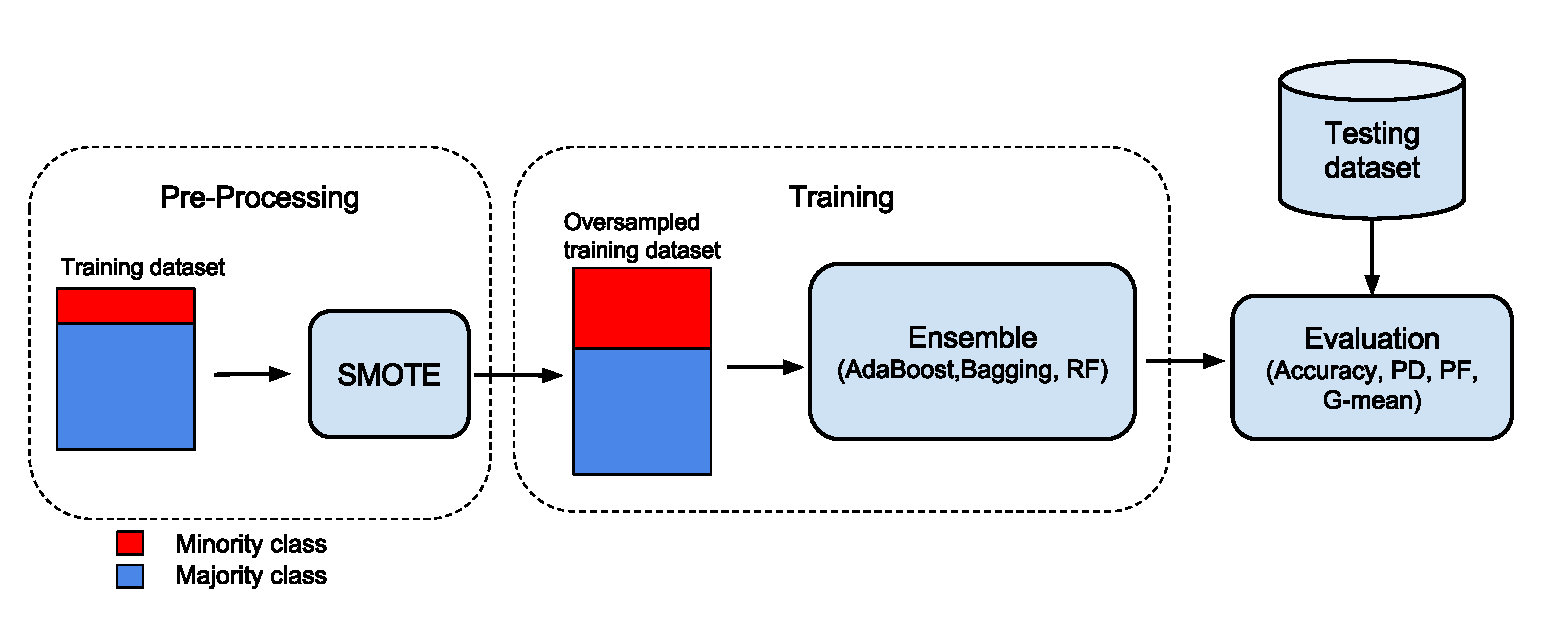
\includegraphics[scale=0.50]{Framework.eps}
\caption{Hybrid SMOTE+Ensemble approach for bug prediction}
\label{fig:fig1}
\end{figure}

\begin{table}[H]
\caption{Datasets Description}
\begin{centering}
\scalebox{0.8}{
\begin{tabular}{c c p{2.5cm} c c c c c c c }
\hline 
Dataset & Language & Description & \#Attributes & LOC & \#Modules & \#Non-defects  & \#Defects & \% Non-defects & \% Defects
\tabularnewline
\hline 
CM1 & C & NASA spacecraft instrument & 22 & 20K & 498 & 449 & 49 & 90.16 & 9.83\tabularnewline
KC1 & C++ & System implementing storage management for receiving and processing
ground data & 22 & 43K & 2109 & 1783 & 326 & 84.54 & 15.45\tabularnewline
JM1 & C & Real-time predictive ground system: Uses simulations to generate predictions & 22 & 315K & 10885 & 8779 & 2106 & 80.65 & 19.35\tabularnewline
PC3 & C & Flight software for earth orbiting satellite metadata & 38 & 40K & 1563 & 1403 & 160 & 89.7 & 10.23\tabularnewline
\hline 
\end{tabular}}
\par\end{centering}
\label{table:data}
\end{table}

\section{Datasets Description}
\label{data}
To facilitate the replication and verification of our experiments, four public benchmark datasets \cite{data6464273} from PROMISE Repository \footnote{http://openscience.us/repo/} were used. These datasets were collected from real software projects by NASA which were developed in C/C++ for spacecraft instrumentation (CM1 dataset), storage management of ground data (KC1 dataset), scientific data processing (JM1 dataset), and satellite flight control (PC3 dataset). A detailed description of of the datasets is given in Table \ref{table:data}.



\section{Model evaluation}
\label{evaluation_criteria}
In order to evalute the performance of the software faults prediction model, we used the confusion matrix that shown in Figure \ref{fig:confusion}, which is a table that is often used to describe the classfication model results. 

\begin{figure}[H]
\centering
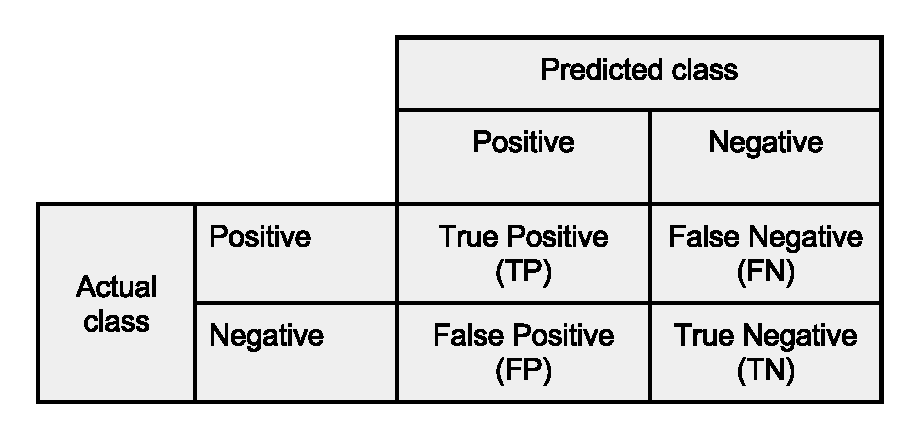
\includegraphics[scale=0.5]{confusion-matrix.eps}
\caption{Confusion matrix}
\label{fig:confusion}
\end{figure}

The defect detection effectiveness is evaluated using four measurements based on the previous confusion matrix; namely, Model Accuracy (Acc), Number of Predicted Defects (PD), Numebr of Incorrectly Predicted cases with No Defects (PF) and G-mean. Acc is the ratio of the correctly predicted faults to the total number of faults. PD is
the ratio of correctly predicted faults to the total number of faults. PF is the number of not fault-prone modules that are predicted incorrectly as defectes. In addtion, we used the G-mean to combine the PD and PF which is a good indicator of the relationship between the two measures. The Acc, PD, PF, G-mean are calculated in Equations \ref{accuracy}, \ref{PD}, \ref{PF}, and \ref{gmean}, respectively.

\begin{small}
\begin{equation}
Accuracy=\frac{TP+TN}{TP + FN + FP + TN}
\label{accuracy}
\end{equation}


\begin{equation}
PD=\frac{TP}{TP+FN}
\label{PD}
\end{equation}

\begin{equation}
PF=\frac{FP}{FP+TN}
\label{PF}
\end{equation}

\begin{equation}
G-mean=\sqrt{PD \times (1-PF)}
\label{gmean}
\end{equation}
\end{small}
%%%%%%%%%%%%%%%%%%%%%%%%%%%%%%%%%%%%%%%%%%%%


%%%%%%%%%%%%%%%%%%%%%%%%%%%%%%%%%%%%%%%%%%%%

%==================================================================
\section{Experiments and Results}
\label{experiments}

The experiments are conducted on three stages; at first, three basic classifiers commonly used in literature are applied and evaluated on the investigated datasets. The classifiers are Naive Bayes (NB), Multilayer Perceptron (MLP) and the C4.5 decision trees. We used the J48 implementation of C4.5 which is available in Weka. In the second stage the ensemble classifiers including RF, Bagging and Adaboosts are applied. Finally, in third stage the hybrid approach of SMOTE combined with best ensemble method in the previous stage is applied and evaluated.

All algorithms in our experiments are applied based on a 10 folds cross-validation as a training and testing methodology. The algorithms are evaluated using the evaluation criteria described in the previous section. As can be seen in Figure  \ref{fig:basic}, evaluation results of basic classifiers show that J48 obtained better results compared to MLP in terms of PD and G-mean for all datasets. While NB tends to give higher FP rates which makes it worst. 



\begin{figure}[H]
\centering
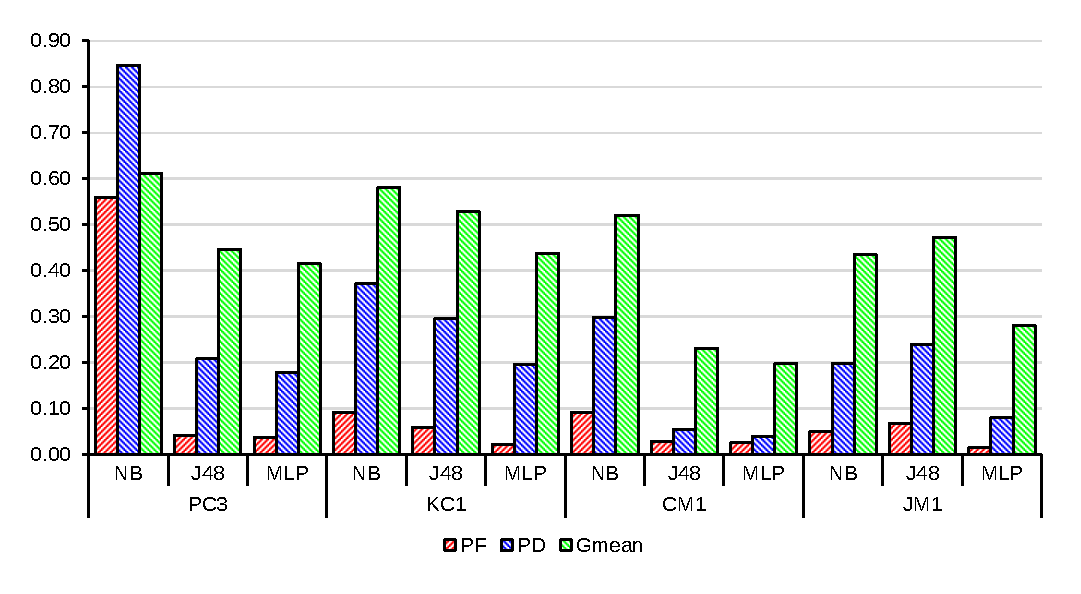
\includegraphics[scale=0.6]{basicresults.eps}
\caption{Evaluation results of basic classifiers.}
\label{fig:basic}
\end{figure}


In the second stage of the experiments, the ensemble classifiers RF, Bagging and Adaboost are applied in attempt to improve the defect detection rates. For Bagging and Adaboost, a base classifier must be selected. In our experiments, J48 is selected to be a base classifier for these two ensembles for three reasons: first due to their good performance compared to NB and MLP networks in the previous stage, second they are much faster to build than the training MLP networks, third it is preferable that the base classifiers are learning algorithms that are highly affected by any change in the training data. 

Number of iterations in ensemble learners could highly affect their performance. Therefore, all ensembles are experimented using different number of iterations starting from 10 up to 100 iterations with a step of 10 iterations increased in each experiment. The best performance of Bagging is obtained with 10 iterations for all datasets. For Adaboost, it was obtained with 10 iterations for PC3 and JM1, and 20 iterations for CM1 and KC1. For RF, the best results are obtained with 30, 50, 60 and 80 for CM1, PC3, JM1 and KC1, respectively. Evaluation results of best ensembles models compared to J48 which was the best in the previous stage are shown in the Figure \ref{fig:ensembles}. It can be seen that Adaboost obtained best results compared to the other classifiers with a noticeable improvement in G-mean and PD rates and very competitive low FP rates.

\begin{figure*}[H]
\centering
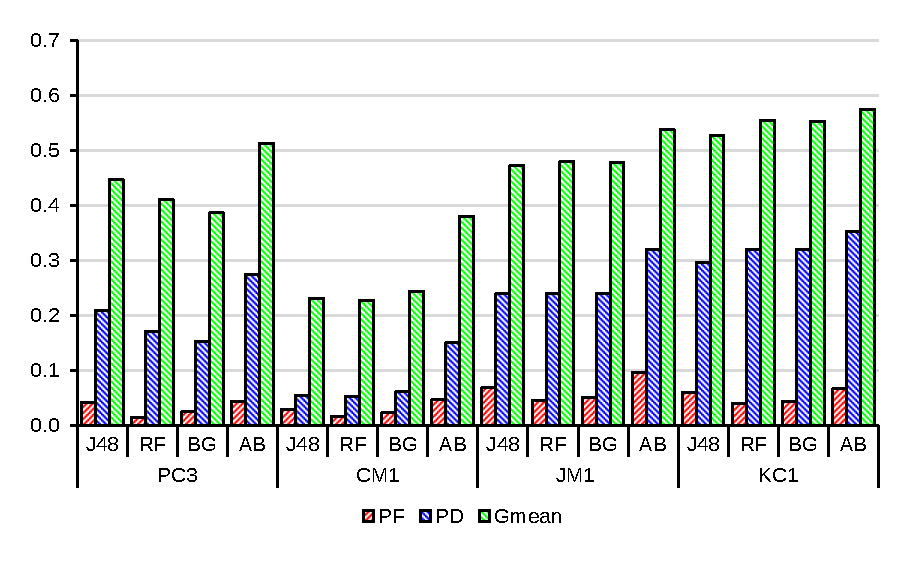
\includegraphics[scale=0.6]{Ensembles.eps}
\caption{Evaluation results of ensemble classifiers and J48 decision tree model.}
\label{fig:ensembles}
\end{figure*}


In the last stage of the experiments, we experiment the effect of combining SMOTE with the best ensemble classifier from the previous stage which is Adaboost. In SMOTE there are two different parameters that influence its performance: number of nearest neighbors ($k$) to use and the percentage of SMOTE instances ($P$) to create. For the first parameters, the default number of 5 neighbors is used which was recommended in \cite{chawla2002smote}. While for the second parameter, different percentages are experimented starting from 20\% up to 200\%. Figure \ref{fig:smote+AB} shows the PD, PF and G-mean evaluation values of Adaboost when trained on datasets oversampled by SMOTE with different $P$ values. According this figure the best performance obtained for CM1 and KC1 datasets is at $P$ of 120\% and for JM1 and PC3 datasets is at 180\% and 200\%, respectively.


 

\begin{figure*}[h]
	\scalebox{0.6}{
		\begin{tabular}{p{2cm} p{5cm} p{4cm} p{5cm} }
			\centering
			
&			\subfigure[CM1]{\label{fig:a}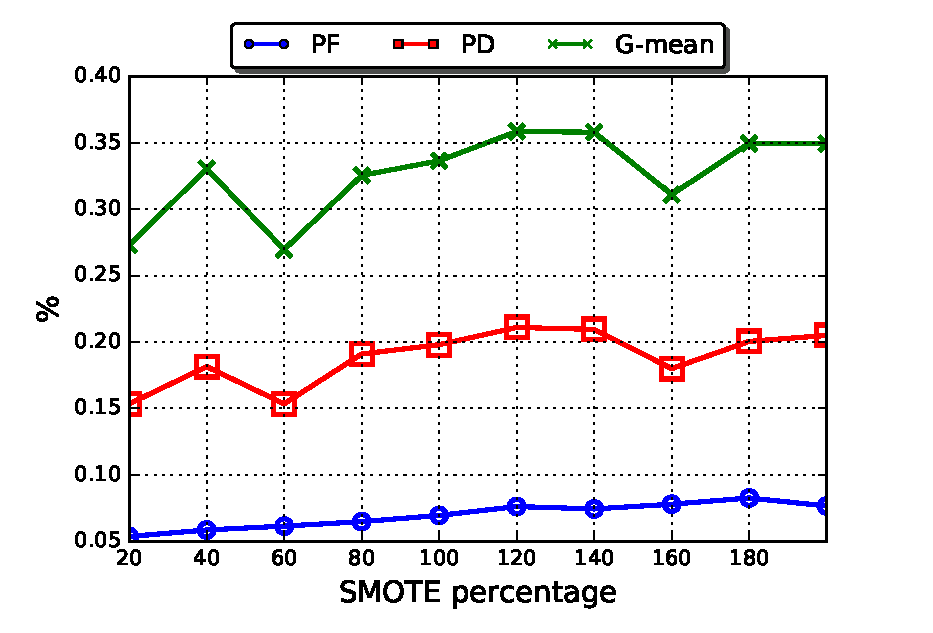
\includegraphics[scale=0.45]{SMOTE-AdaBoost-CM1}}& &
			\subfigure[JM1]{\label{fig:a}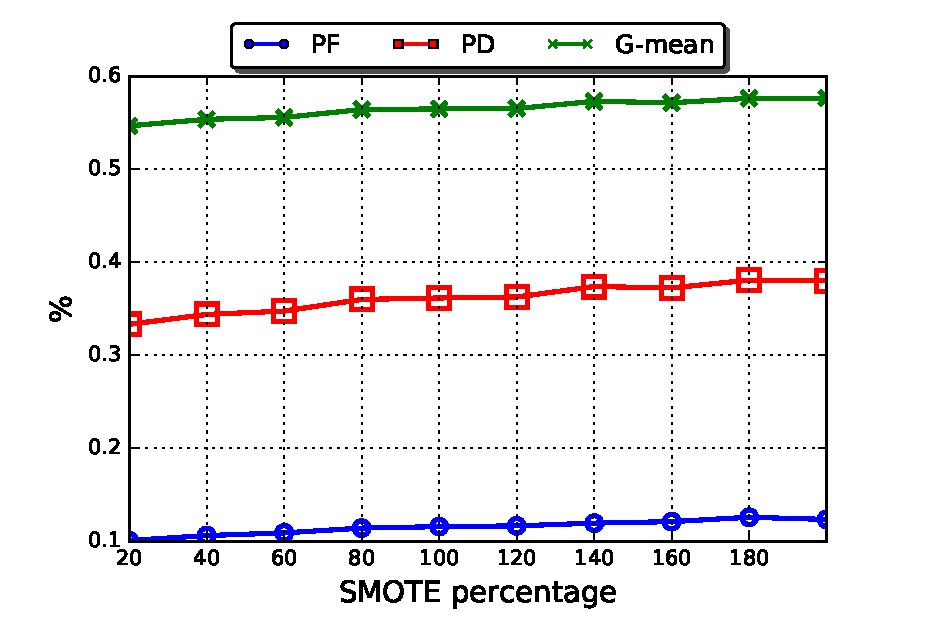
\includegraphics[scale=0.45]{SMOTE-AdaBoost-JM1}}

			\vspace{-1.0in}
			\\
&			\subfigure[KC1]{\label{fig:a}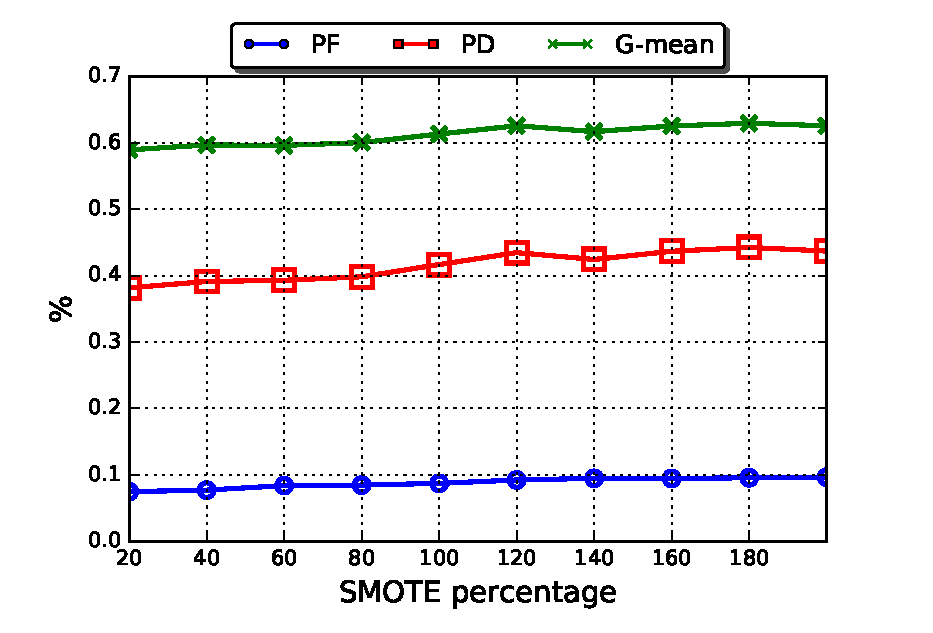
\includegraphics[scale=0.45]{SMOTE-AdaBoost-KC1}}& &
			\subfigure[PC3]{\label{fig:a}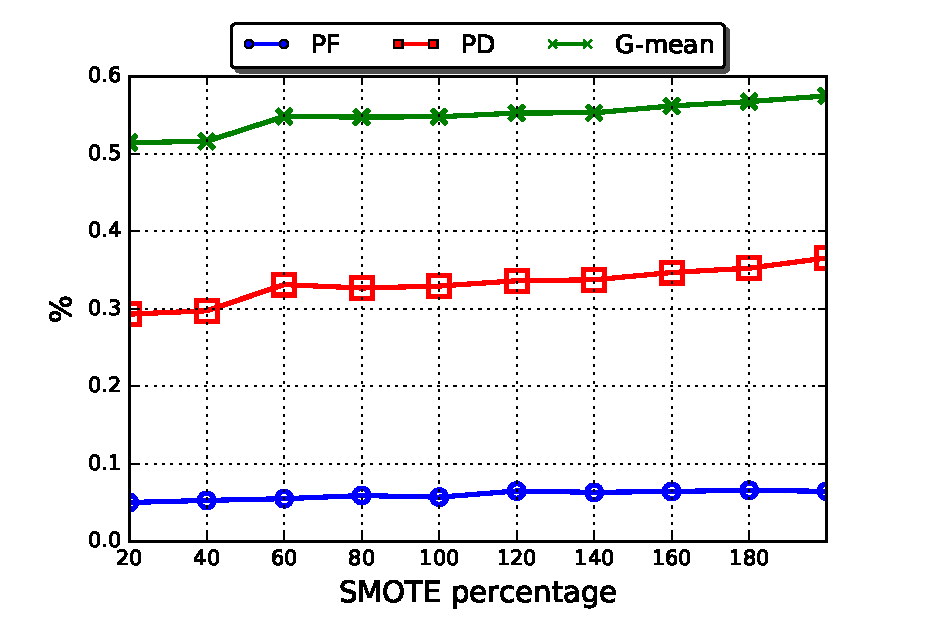
\includegraphics[scale=0.45]{SMOTE-AdaBoost-PC3}}

			\vspace{-1.0in}
			\\
%				
		\end{tabular}
	}
	\caption{Evaluation results of SMOTE+AdaBoost by changing number of iterations.}
	\label{fig:smote+AB}
	\vspace{-0.0in}
\end{figure*}



Finally, the best obtained results of SMOTE combined Adaboost with all other classifiers are shown in Table \ref{table:PC3results}, \ref{table:KC1results}, \ref{table:CM1results} and \ref{table:JM1results}, for PC3, KC1, CM1, JM1 datasets respectively. In JM1 and KC1 datasets, the SMOTE+Adaboost approach managed to achieve best results in terms of PD and G-mean with very competitive low PF rate. For PC3 dataset, we can see that although NB has the best results in terms of PD and G-mean, it has the worst FP rate which is very high at value of 55.89\%. On the other hand, SMOTE+Adaboost comes second with 36.56\%  for PD and 57.48\% for G-mean with low FP rate of 6.45\% which makes more favorable. For CM1, it can be seen that SMOTE enhanced the performance of Adaboost in all criteria but it comes second after NB. 



\begin{table}[H]
\caption{Evaluation results for PC3 dataset}
\begin{centering}
\scalebox{0.7}{
\begin{tabular}{l c c c c}
\hline 
 & Accuracy & PF & PD & G-mean\tabularnewline
\hline 
NB & 0.4826 & 0.5589 & 0.8469 & 0.6112\tabularnewline
J48 & 0.8814 & 0.0418 & 0.2081 & 0.4466\tabularnewline
MLP & 0.8820 & 0.0378 & 0.1788 & 0.4147\tabularnewline
RF & 0.9018 & 0.0149 & 0.1713 & 0.4107\tabularnewline
Bagging & 0.8912 & 0.0247 & 0.1531 & 0.3865\tabularnewline
AdaBoost & 0.8869 & 0.0433 & 0.2750 & 0.5129\tabularnewline
SMOTE+AdaBoost & 0.8772 & 0.0645 & 0.3656 & 0.5748\tabularnewline
\hline 
\end{tabular}}
\par\end{centering}
\label{table:PC3results}
\end{table}


\begin{table}[H]
\caption{Evaluation results for KC1 dataset}
\begin{centering}
\scalebox{0.7}{
\begin{tabular}{l c c c c}
\hline 
 & Accuracy & PF & PD & G-mean\tabularnewline
\hline 
NB & 0.8246 & 0.0925 & 0.3715 & 0.5806\tabularnewline
J48 & 0.8404 & 0.0601 & 0.2964 & 0.5278\tabularnewline
MLP & 0.8565 & 0.0229 & 0.1963 & 0.4380\tabularnewline
RF & 0.8610 & 0.0402 & 0.3208 & 0.5548\tabularnewline
Bagging & 0.8582 & 0.0434 & 0.3200 & 0.5533\tabularnewline
AdaBoost & 0.8438 & 0.0665 & 0.3534 & 0.5743\tabularnewline
SMOTE+AdaBoost & 0.8329 & 0.0957 & 0.4424 & 0.6294\tabularnewline
\hline 
\end{tabular}}
\par\end{centering}
\label{table:KC1results}
\end{table}


\begin{table}[H]
\caption{Evaluation results for CM1 dataset}
\begin{centering}
\scalebox{0.7}{
\begin{tabular}{l c c c c}
\hline 
 & Accuracy & PF & PD & G-mean\tabularnewline
\hline 
NB & 0.8484 & 0.0918 & 0.2985 & 0.5207\tabularnewline
J48 & 0.8805 & 0.0294 & 0.0550 & 0.2310\tabularnewline
MLP & 0.8825 & 0.0256 & 0.0400 & 0.1974\tabularnewline
RF & 0.8920 & 0.0165 & 0.0525 & 0.2272\tabularnewline
Bagging & 0.8865 & 0.0234 & 0.0610 & 0.2441\tabularnewline
AdaBoost & 0.8743 & 0.0468 & 0.1510 & 0.3794\tabularnewline
SMOTE+AdaBoost & 0.8536 & 0.0762 & 0.2110 & 0.3585\tabularnewline
\hline 
\end{tabular}}
\par\end{centering}
\label{table:CM1results}
\end{table}

\begin{table}[H]
\caption{Evaluation results for JM1 dataset}
\begin{centering}
\scalebox{0.7}{
\begin{tabular}{l c c c c}
\hline 
 & Accuracy & PF & PD & G-mean\tabularnewline
\hline 
NB & 0.8042 & 0.0507 & 0.1993 & 0.4350\tabularnewline
J48 & 0.7973 & 0.0688 & 0.2394 & 0.4722\tabularnewline
MLP & 0.8100 & 0.0148 & 0.0799 & 0.2806\tabularnewline
RF & 0.8167 & 0.0450 & 0.2402 & 0.4789\tabularnewline
Bagging & 0.8118 & 0.0511 & 0.2406 & 0.4778\tabularnewline
AdaBoost & 0.7912 & 0.0958 & 0.3199 & 0.5378\tabularnewline
SMOTE+AdaBoost & 0.7787 & 0.1259 & 0.3808 & 0.5764\tabularnewline
\hline 
\end{tabular}}
\par\end{centering}
\label{table:JM1results}
\end{table}



\section{Conclusions}
\label{conclusion}

Delivering high quality software products on time within budgetary cost is crucial issue for the success of software companies. In order to help software developers in undertaking this issue, an attempt has been made in this paper for software defect prediction.

This paper formulates the software defect prediction problem as a classification task. It further investigates the impact of several
ensemble methods to solve the defect prediction problem. Specifically, we have developed a hybrid ensemble classification based on over-sampled approach for detecting software defects in different imbalanced datasets. High imbalanced distribution of classes in datasets deteriorates the performance of classification approaches. The proposed approach is developed based on the Synthetic Minority Over-sampling Technique (SMOTE). The experiments have shown that the proposed SMOTE+Ensembles approach has better quality results than the other classification algorithms. Our future research will include the verification of the proposed method on other datasets.






\bibliographystyle{splncs}
\bibliography{ref}
\end{document}
